% !TeX program = xelatex
\documentclass[aspectratio=169,10pt]{beamer}
\usetheme[progressbar=frametitle,numbering=fraction,sectionpage=none]{metropolis}
\usepackage{fontspec}
\usepackage{booktabs}
\usepackage{tikz}
\usetikzlibrary{arrows.meta,positioning}
\setsansfont{Noto Sans CJK SC}
\XeTeXlinebreaklocale "zh"
\XeTeXlinebreakskip=0pt plus 1pt
\definecolor{ink}{HTML}{23373B}
\definecolor{paper}{HTML}{FAFAF7}
\definecolor{teal}{HTML}{116D68}
\definecolor{amber}{HTML}{D28228}
\setbeamercolor{normal text}{fg=ink,bg=paper}
\setbeamercolor{frametitle}{fg=white,bg=ink}
\setbeamercolor{alerted text}{fg=teal}
\setbeamercolor{progress bar}{fg=amber,bg=ink!18}
\setbeamertemplate{navigation symbols}{}
\setlength{\parskip}{3pt}
\graphicspath{{figures/}}
\newcommand{\credit}[1]{\par\vspace{2pt}{\scriptsize\color{ink!75}#1}\par}
\newcommand{\point}[2]{\par\textcolor{teal}{\textbf{#1}}\par #2\par\vspace{3pt}}
\newcommand{\talk}[2]{\note{#1\par #2}}
\newcommand{\paperone}{Xie, Hao \& Xie, Frontiers in Public Health (2025). \href{https://doi.org/10.3389/fpubh.2025.1647200}{10.3389/fpubh.2025.1647200}}
\newcommand{\papertwo}{Xie, Hao \& Xie, Computational Statistics (2026). \href{https://doi.org/10.1007/s00180-026-01760-4}{10.1007/s00180-026-01760-4}}
\newcommand{\nolte}{Nolte, S. (2024). \textit{More Than Just Associations: An Introduction to Causal Inference for Sport Science}. 硕士论文，德国科隆体育大学。}
\tikzset{factor/.style={draw=teal!60,fill=teal!7,rounded corners=2pt,inner sep=6pt,align=center},patharrow/.style={-{Stealth},semithick,draw=teal}}
\title{运动训练负荷的因果分析}
\subtitle{从跑者损伤路径到可穿戴生理时序}
\author{谢淘}
\institute{高校教师岗位科研汇报}
\date{}
% To show speaker notes, uncomment the following line and recompile.
% \setbeameroption{show notes}
\begin{document}

\begin{frame}[plain]
  \relax{\usebeamerfont{title}\inserttitle\par}
  \smallskip
  {\usebeamerfont{subtitle}\insertsubtitle\par}
  \medskip
  {\color{amber}\rule{.19\textwidth}{1.5pt}}\par
  \bigskip
  \insertauthor\par
  \insertinstitute
  \talk{00:00–00:25}{各位老师好，我是谢淘。我的研究围绕运动训练负荷、恢复与运动损伤展开。今天先从体育科学为什么需要因果证据讲起，再说明为什么训练决策需要因果推断，随后介绍两篇论文的方法、主要发现，以及入职后的验证计划。}
\end{frame}

\section{研究方向}
\begin{frame}{研究方向｜运动负荷、恢复与损伤的因果分析}
\begin{columns}[T,onlytextwidth]
\column{.31\textwidth}
\point{现状｜训练决策需要干预证据}{体育科学常问：更换训练方案后，运动表现或损伤会怎样？随机对照试验在高水平运动等实际场景中往往难以实施，因此研究也依赖训练日志等观察数据。}
\column{.31\textwidth}
\point{问题｜组间差异难以解释}{同一运动员在同一时期只能接受其中一种策略。观察到的高、低负荷组可能在赛程、伤病史和恢复条件上已有差异。}
\column{.31\textwidth}
\point{路径｜把干预问题写清楚}{先定义人群、策略和结局，再用专业知识构建因果图，明确比较所依赖的假设，估计效应并检验稳健性。}
\end{columns}
\begin{alertblock}{我的切入点}
从跑者日志与可穿戴时序出发，识别负荷、恢复和损伤的候选路径，并在纵向队列和训练干预中验证。
\end{alertblock}
\credit{研究方向的文献依据｜Nolte (2024)，Introduction，§1.1–1.3，正文第 1–4 页。}
\talk{00:25–01:20}{Simon Nolte 在硕士论文的引言中把实证研究区分为描述、预测与因果推断。体育研究很多时候希望改变训练或战术，但运动员不一定能接受随机分组，因此常要从观察数据出发。最难的是，同一个人在同一时期只能接受一种策略，另一种策略下的结局看不到。Nolte 提出用领域知识和因果图说明假设，再估计目标效应并检验稳健性。我的研究把这个问题落到训练负荷、恢复和运动损伤。}
\end{frame}

\begin{frame}{研究方向｜冲刺组损伤更多，能否建议减少冲刺？}
\begin{columns}[T,onlytextwidth]
\column{.49\textwidth}
\textbf{示意｜赛程密度是潜在混杂因素}
\begin{center}
\begin{tikzpicture}[font=\small]
\node[factor] (c) at (0,1.32) {赛程密度};
\node[factor] (x) at (-1.45,0) {冲刺跑量 $X$};
\node[factor] (y) at (1.45,0) {后续损伤 $Y$};
\draw[patharrow] (c) -- (x);
\draw[patharrow] (c) -- (y);
\draw[patharrow,dashed] (x) -- (y);
\end{tikzpicture}
\end{center}
\small 虚线是待检验路径。密集赛程可能同时改变冲刺暴露与恢复机会。
\column{.47\textwidth}
\point{相关性}{比较实际高、低负荷组的损伤风险。组间差异可能包含赛程或既往伤病的影响。}
\point{预测}{用冲刺量和其他信息预测下一周谁更可能受伤。}
\point{因果效应}{比较同一目标人群采用两种冲刺策略后，下一周的损伤风险。}
\end{columns}
\medskip
\[
\underbrace{P(Y{=}1\mid X{=}x_H)-P(Y{=}1\mid X{=}x_L)}_{\text{观察组差}}
\qquad
\underbrace{P(Y{=}1\mid do(X{=}x_H))-P(Y{=}1\mid do(X{=}x_L))}_{\text{干预风险差}}
\]
\credit{示意中高、低策略及随访窗口须在研究中预先定义。}
\talk{01:20–02:15}{假设冲刺多的队员受伤也更多，教练会问，减少冲刺有用吗？赛程密集可能同时带来更多冲刺和更少恢复，造成组间差异。观察组差描述实际被分到高低负荷组的人；干预风险差则比较同一目标人群采用两种负荷策略之后会怎样。两种策略要能实施，暴露应先于结局，且要有足够可比的人。预测准确、变量发生在前，或图里出现一条边，都不足以单独识别这种干预效应。}
\end{frame}

\section{研究内容}
\begin{frame}{研究内容｜用两类数据回答两个互补问题}
\begin{columns}[T,onlytextwidth]
\column{.47\textwidth}
\point{研究一｜不同负荷等级与损伤如何相连？}{\textbf{数据}：跑者训练日志单日子集，42,766 条样本。\par
\textbf{方法}：用分位数阈值（QTF）构造有序等级，拟合潜在高斯有向无环图。\par
\textbf{输出}：候选路径与等级变化下的模型损伤概率差。}
\column{.47\textwidth}
\point{研究二｜活动效应怎样跨时间传递？}{\textbf{数据}：模拟序列与 30 位 Fitbit 使用者的分钟级序列。\par
\textbf{方法}：TS-ICD 以时间先后约束图搜索，再用中介模型分解候选路径。\par
\textbf{输出}：部分祖先图、条件独立检验次数及间接效应估计。}
\end{columns}
\begin{alertblock}{两项研究的分工}
研究一处理负荷分级与损伤；研究二处理滞后结构，实际分析结局为心率。
\end{alertblock}
\credit{\paperone\par\papertwo}
\talk{02:15–03:05}{两项研究解决的是两个不同的数据问题。第一项把连续训练指标转换成可比较的有序等级，再用潜在高斯模型估计图结构和候选效应。第二项保留分钟级时间信息，限制未来指向过去的候选关系，然后对强度、步数和心率之间的路径做中介分析。这为后续校园足球研究提供了两种可衔接的方法：前者回答该看哪些变量，后者回答该看哪段历史。}
\end{frame}

\section{研究结果}
\begin{frame}{研究结果一｜冲刺与恢复是优先验证的损伤路径}
\begin{columns}[T,onlytextwidth]
\column{.55\textwidth}
\centering
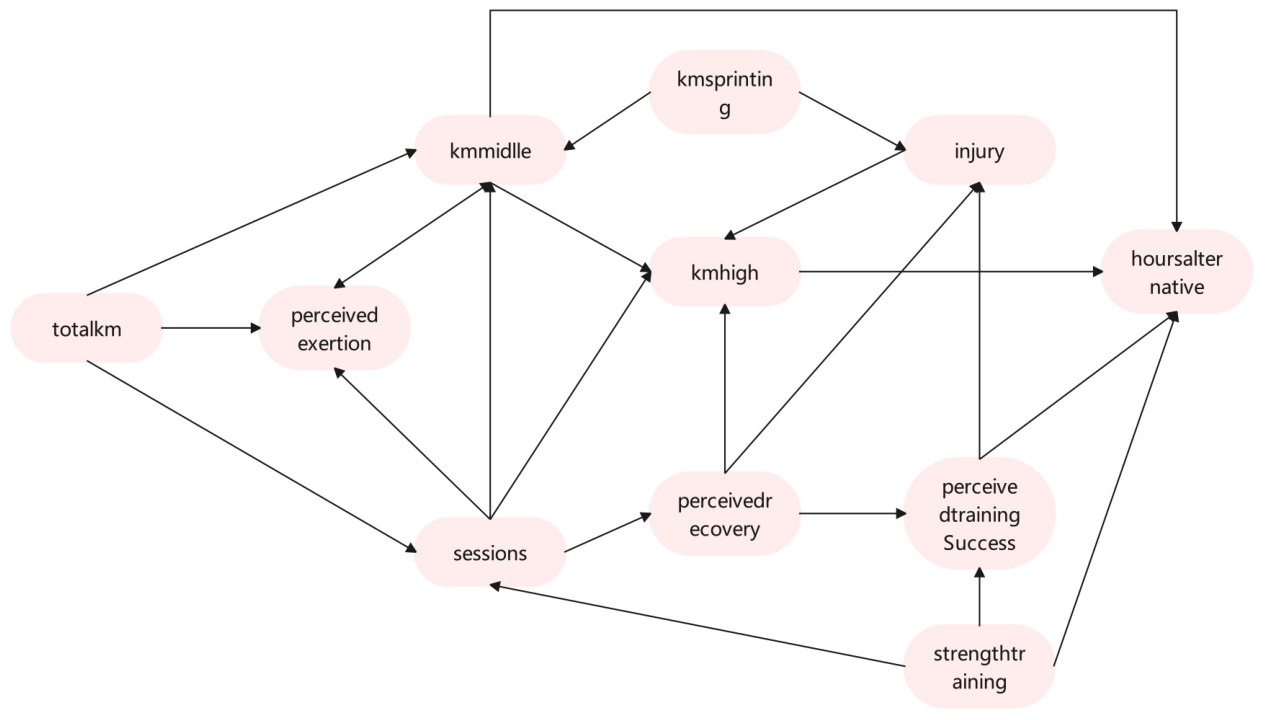
\includegraphics[width=\linewidth,height=.59\textheight,keepaspectratio]{dag.png}
\credit{原论文图 4｜重采样估计的部分有向图（CPDAG）。}
\column{.42\textwidth}
\point{3 条直接路径}{冲刺跑量、主观恢复与主观训练成效在估计图中直接连接损伤。}
\point{2 条间接路径}{总跑量经训练频次与恢复连接损伤；力量训练经主观训练成效连接损伤。}
\point{本人贡献}{第一作者、通讯作者。承担研究构思、数据整理及初稿撰写。}
\end{columns}
\credit{\paperone · 图 4，CC BY。}
\talk{03:05–04:00}{先在原图里找到 Injury。论文报告了三条直接和两条间接路径。值得进一步跟踪的一条是，总跑量经训练频次与主观恢复和损伤相连。它提示采集队列时要同时记录训练次数与恢复，而只记录总量会丢掉路径信息。图里有方向未完全确定的边，而且单日观察不能充分判断负荷先于损伤，故这些边首先用于提出要验证的关系。}
\end{frame}

\begin{frame}{研究结果一｜低到中、高等级的转换更值得追踪}
\begin{columns}[T,onlytextwidth]
\column{.55\textwidth}
\centering
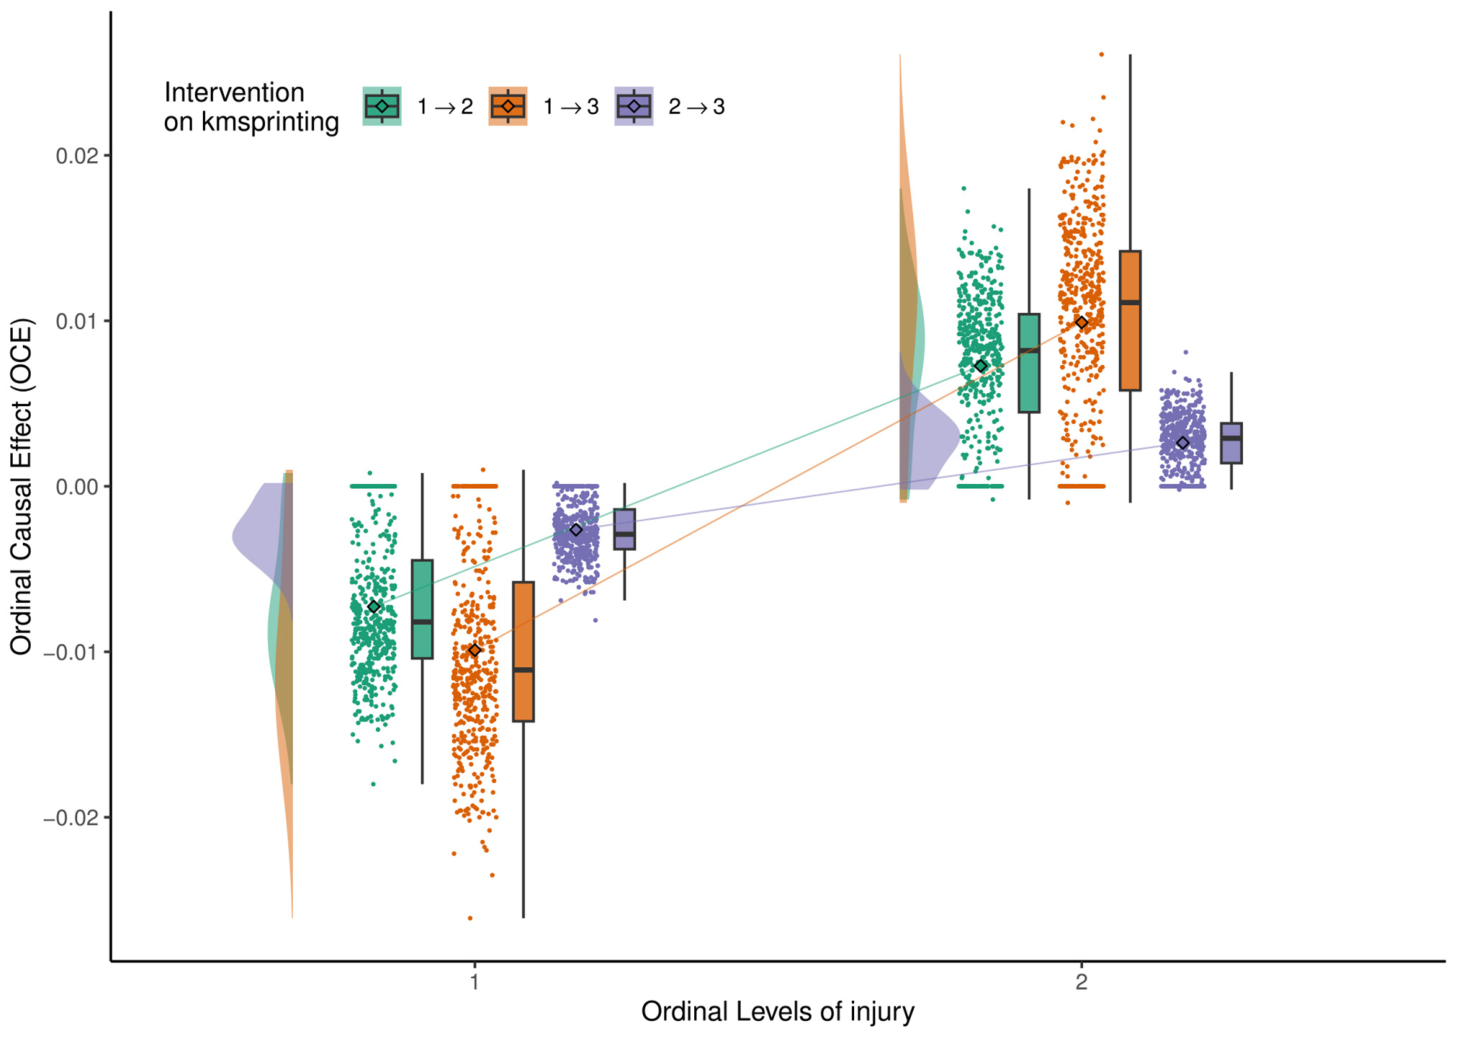
\includegraphics[width=\linewidth,height=.62\textheight,keepaspectratio]{oce.png}
\credit{原论文图 5｜冲刺跑量等级变化的有序效应估计。}
\column{.41\textwidth}
\point{读图}{看 \texttt{Injury = 2}（受伤）对应的分布。正值表示模型估计的损伤概率上升。}
\point{结果}{低 $\to$ 中、低 $\to$ 高时估计偏正；中 $\to$ 高时的估计更接近零。}
\point{下一步}{用赛季随访明确时间顺序，再检查分级阈值和效应能否迁移。}
\end{columns}
\credit{\paperone · 图 5，CC BY。}
\talk{04:00–04:45}{图5不是直接比较不同人群的损伤比例，而是给出图模型下等级变化时估计的概率差。请看受伤类别中的转换分布。低到中或高的估计偏正，中到高的估计更靠近零。这里强调的是随访验证的优先级。由于数据来自单日子集，效应依赖图结构和混杂处理假设，阶段阈值还需要在独立样本上检验。}
\end{frame}

\begin{frame}{研究结果二｜时间约束减少了图搜索所需的检验}
\begin{columns}[T,onlytextwidth]
\column{.62\textwidth}
\centering
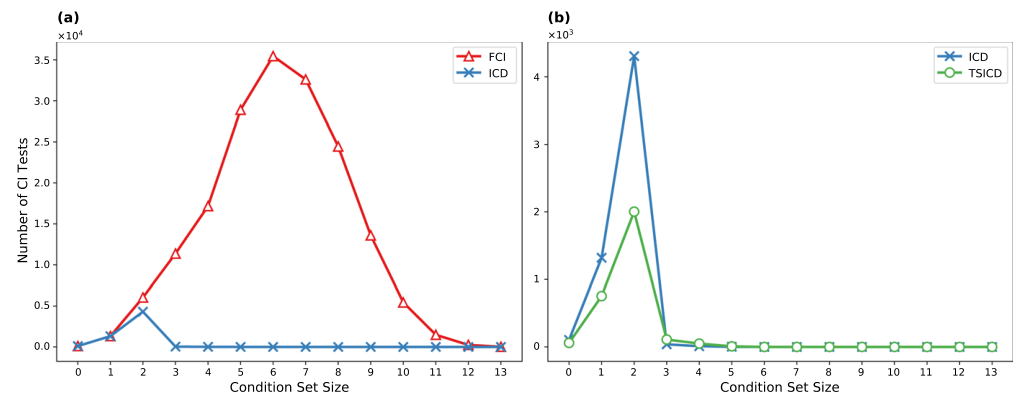
\includegraphics[width=\linewidth,height=.58\textheight,keepaspectratio]{ci.png}
\credit{原论文图 2｜左：FCI 与 ICD。右：ICD 与 TS-ICD。两图纵轴量级不同。}
\column{.35\textwidth}
\point{效率}{在论文比较设置下，加入时序约束的 TS-ICD 所需条件独立检验次数最少。}
\point{结构}{在模拟数据中检验结构恢复；时序约束排除违反先后顺序的方向。}
\point{本人贡献}{共同第一作者（署名第一）。承担设计、方法提出、分析、制图和撰稿。}
\end{columns}
\credit{\papertwo · 图 2。}
\talk{04:45–05:40}{图2的横轴是条件集规模，纵轴是条件独立检验次数。左图比较FCI和ICD，两者差别尤其明显；右图比较ICD和加入时间约束的TS-ICD。两个面板的纵轴量级不同，适合在同一面板内读曲线。结果表明，明确时间先后可以减少检验，并使结构满足时间顺序。这不是用检验次数证明因果方向，而是在限定的搜索规则和设定中提高计算效率。}
\end{frame}

\begin{frame}{研究结果二｜强度和步数通过不同路径关联心率}
\begin{columns}[T,onlytextwidth]
\column{.48\textwidth}
\point{滞后强度 → 近期及当前强度 → 心率}{合计间接效应 \alert{11.582}，约占估计总效应的 \alert{73\%}。}
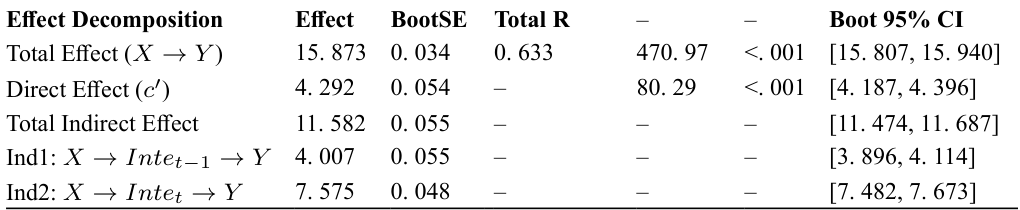
\includegraphics[width=\linewidth]{lagtable.png}
\credit{原论文表 3 · 效应分解节选。}
\column{.48\textwidth}
\point{滞后步数 → 代谢当量（METs）→ 心率}{间接效应 \alert{0.393}（95\% CI 0.389–0.396）；直接效应 $p=0.606$。}
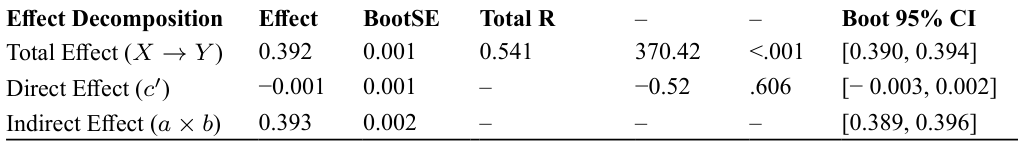
\includegraphics[width=\linewidth]{mettable.png}
\credit{原论文表 4 · 效应分解节选。}
\end{columns}
\begin{alertblock}{结果的适用范围}
330,842 条时间窗观测来自 30 人。估计量依赖模型设定，直接效应未检出；损伤结局有待新队列检验。
\end{alertblock}
\credit{\papertwo}
\talk{05:40–06:35}{表3把两分钟前的活动强度与当前心率之间的估计总效应分解。经近期和当前强度的两条路径合计约占百分之七十三。表4中，滞后步数经代谢当量的间接效应为零点三九三，直接效应没有达到统计显著。这提示穿戴数据分析应保留活动历史，也应同时看步数与代谢需求。三十三万余条是时间窗，不是独立参与者。本研究的结局是心率，未来才检验对损伤监测的价值。}
\end{frame}

\section{入职科研计划}
\begin{frame}{后续研究｜在校园足球中检验负荷与恢复路径}
\point{研究问题}{负荷波动是否经次日恢复与后续损伤相连？该关系在不同队伍、赛季及训练阶段是否稳定？}
\begin{columns}[T,onlytextwidth]
\column{.49\textwidth}
\point{前瞻队列}{基线记录既往损伤与训练水平；每次训练记录时长、主观用力和训练内容；次日随访恢复。条件允许时对设备子样本保留时间戳与处理参数。}
\column{.47\textwidth}
\point{结局与分析}{以每千暴露小时损伤率为主要结局，跟踪踝扭伤与缺训。预设混杂与滞后窗口，按队伍或赛季留出验证，评估校准和路径稳定性。}
\end{columns}
\credit{拟开展研究｜采集前完成伦理审批、知情同意与伤例判定规范。}
\talk{06:35–07:40}{我会先与校园足球队或课程做前瞻试点。先定义一次暴露的起止、次日恢复的记录窗口以及损伤和缺训标准。设备子样本保存原始记录与处理规则，以便比较窗口选择的影响。对模型验证，按队伍或赛季留出数据，避免重复记录泄漏。第一步看不同阶段的负荷、恢复和损伤是否有稳定的时间关系，再根据可测量的混杂、数据规模和事件数选择效应分析。}
\end{frame}

\begin{frame}{后续研究｜用队伍层面的试点评估预防方案}
\point{比较方案}{常规训练 vs. 负荷反馈结合踝部神经肌肉热身。合作队伍充足时按队分组，以减少方案互相影响。}
\point{判定顺序}{先评价招募、记录完整性、依从性与安全，再估计损伤发生率、率比或缺训天数的变化及区间。}
\smallskip
\begin{tabular}{@{}lp{.76\textwidth}@{}}
\toprule
阶段 & 研究任务与可交付成果\\
\midrule
第 1 年 & 完成伦理、合作与数据采集试点，形成数据字典与质量报告。\\
第 2 年 & 做纵向及跨赛季验证，形成可复现分析与投稿稿件。\\
第 3 年 & 完成预防方案可行性试点，形成教练反馈报告与可复制流程。\\
\bottomrule
\end{tabular}
\credit{正式样本量依据试点估计；队伍或事件数不足时，以可行性和数据质量为交付。}
\talk{07:40–09:15}{干预阶段拟比较两种可执行方案：常规训练，以及加入负荷反馈与踝部神经肌肉热身的训练。方案包含两个组成部分，试点估计的是组合方案的效果。优先看教练能不能落实、随访与记录能否完成、是否出现安全问题。队伍少时不以显著性作为试点成功的标准。第一年建立记录，第二年验证候选路径和模型迁移，第三年把负荷反馈和热身流程带回训练中。数据采集和质量控制也可以连接足球教学与学生科研训练。}
\end{frame}

\begin{frame}{结论｜两项成果为校园足球预防研究提供方法基础}
\point{跑者训练日志}{以有序变量因果图提出冲刺负荷与恢复相关的候选损伤路径。}
\point{可穿戴生理时序}{通过时间约束降低图搜索开销，并分解活动强度与心率的滞后路径。}
\point{下一步}{用校园足球的前瞻记录检验路径，在设计明确的训练比较中评价预防方案。}
\medskip
{\Large 谢谢各位老师}
\talk{09:15–10:00}{我的研究从体育训练干预问题出发，区分了观察关联、预测与改变训练的效果。第一项研究用跑者日志定位值得先监测的暴露和恢复指标；第二项研究用时序约束说明应该保留哪些历史信息。基于这两项已发表成果，我拟用校园足球的前瞻队列检验路径，再通过方案比较评价可执行性和损伤结局。谢谢各位老师，欢迎提问。}
\end{frame}

\appendix
\section{答辩备查}
\begin{frame}{备查｜个人科研积累与成果范围}
\point{体育训练与足球专项}{庆一大学体育训练博士阶段；本硕足球专项，曾承担公共体育足球课程教学。}
\point{博士阶段科研参与}{按本人简历，参与青少年足球成熟度与损伤、强化学习动作纠正反馈、外侧踝扭伤风险因素研究的数据或资料整理分析。}
\point{方法积累与在审拓展}{第一作者 ACM 会议论文以 Apriori 分析足球比赛；简历另列跑者损伤与训练的中介研究、足球预期进球模型比较两项在审工作。}
\credit{ACM 会议论文 DOI \href{https://doi.org/10.1145/3603273.3631190}{10.1145/3603273.3631190}。庆一大学项目立项信息尚未独立核验。}
\end{frame}

\begin{frame}{备查｜从观察数据到训练策略效应的识别条件}
\point{可比性与可实施性}{先明确策略、入组时间和随访期。在可测混杂条件下比较并检验暴露重叠；有条件时用随机设计。}
\point{中介与时变混杂}{区分基线伤病与负荷之后的恢复；如果恢复影响下一期训练，普通回归控制恢复可能改变目标估计量。}
\point{统计不确定性与迁移}{考虑同一运动员和队伍内相关；对缺失、滞后窗口、阈值及赛季阶段做敏感性分析。}
\end{frame}

\begin{frame}{主要来源}
\small
\point{研究方向的文献起点}{\nolte\par
依据 Introduction 的 Relevance、Previous Research 和 Aim；因果图例为本汇报自绘。}
\point{两篇代表性成果}{\paperone\par\papertwo}
\point{演示模板}{\href{https://github.com/josephwright/beamer}{LaTeX Beamer} 与 \href{https://github.com/matze/mtheme}{Metropolis} 学术演示主题。}
\end{frame}
\end{document}
